
This example investigates properties of various traces. 

\subsubsection{Rectangle}
Markers in \cref{fig:0012-r} shows the variation of the eigenvalues of the generalized shear correction matrix \eqref{eq:shear-correction} for different Poisson ratios \(\nu\) and aspect ratios $d/b$.
Curves are shown for the equations in \cref{tab:rectangle-scf}.

\begin{subequations}\label{eq:scf-rectangle}
\renewcommand{\theequation}{\theparentequation\alph{equation}}%
\begin{table}[h]
  \renewcommand{\arraystretch}{1.5} 
  \centering
  \caption{Shear correction factors $\kappa$ for a rectangular section.}
  \label{tab:rectangle-scf}
  \begin{tabular}{@{} l p{0.5\linewidth} r @{}}
    \toprule
    \textbf{Reference} & \textbf{Formula} & \textbf{Eq.}\\
    \midrule
     \cite{timoshenko1921correction} 
     & \(\dfrac{2}{3}\)
     & \refstepcounter{equation}(\theequation)\label{eq:scf-rectangle-timo21} 
    \\%[0.8cm]
     \cite{timoshenko1922transverse} 
     & \(\dfrac{5+5 \nu}{6+5 \nu}\) 
     & \refstepcounter{equation}(\theequation)\label{eq:scf-rectangle-timo22} 
    \\%[0.8cm]
     \cite{cowper1966shear}
     & \(\dfrac{10(1+\nu)}{12+11 \nu}\)
     & \refstepcounter{equation}(\theequation)\label{eq:scf-rectangle-cowp66} 
    \\%[0.8cm]
    \cite{renton1991generalized}
    & \(\left[6/5+\left(\frac{\nu}{1+\nu}\right)^2 \sum_{m=0}^{\infty} \sum_{n=1}^{\infty} \frac{144(b / d)^4}{\pi^6(2 m+1)^2 n^2\left[(2 m+1)^2(b / 2 d)^2+n^2\right]}\right]^{-1}\)
    & \refstepcounter{equation}(\theequation)\label{eq:scf-rectangle-rent91} 
    \\
    \bottomrule
  \end{tabular}
\end{table}
\end{subequations}

\begin{figure}[H]
    \centering
    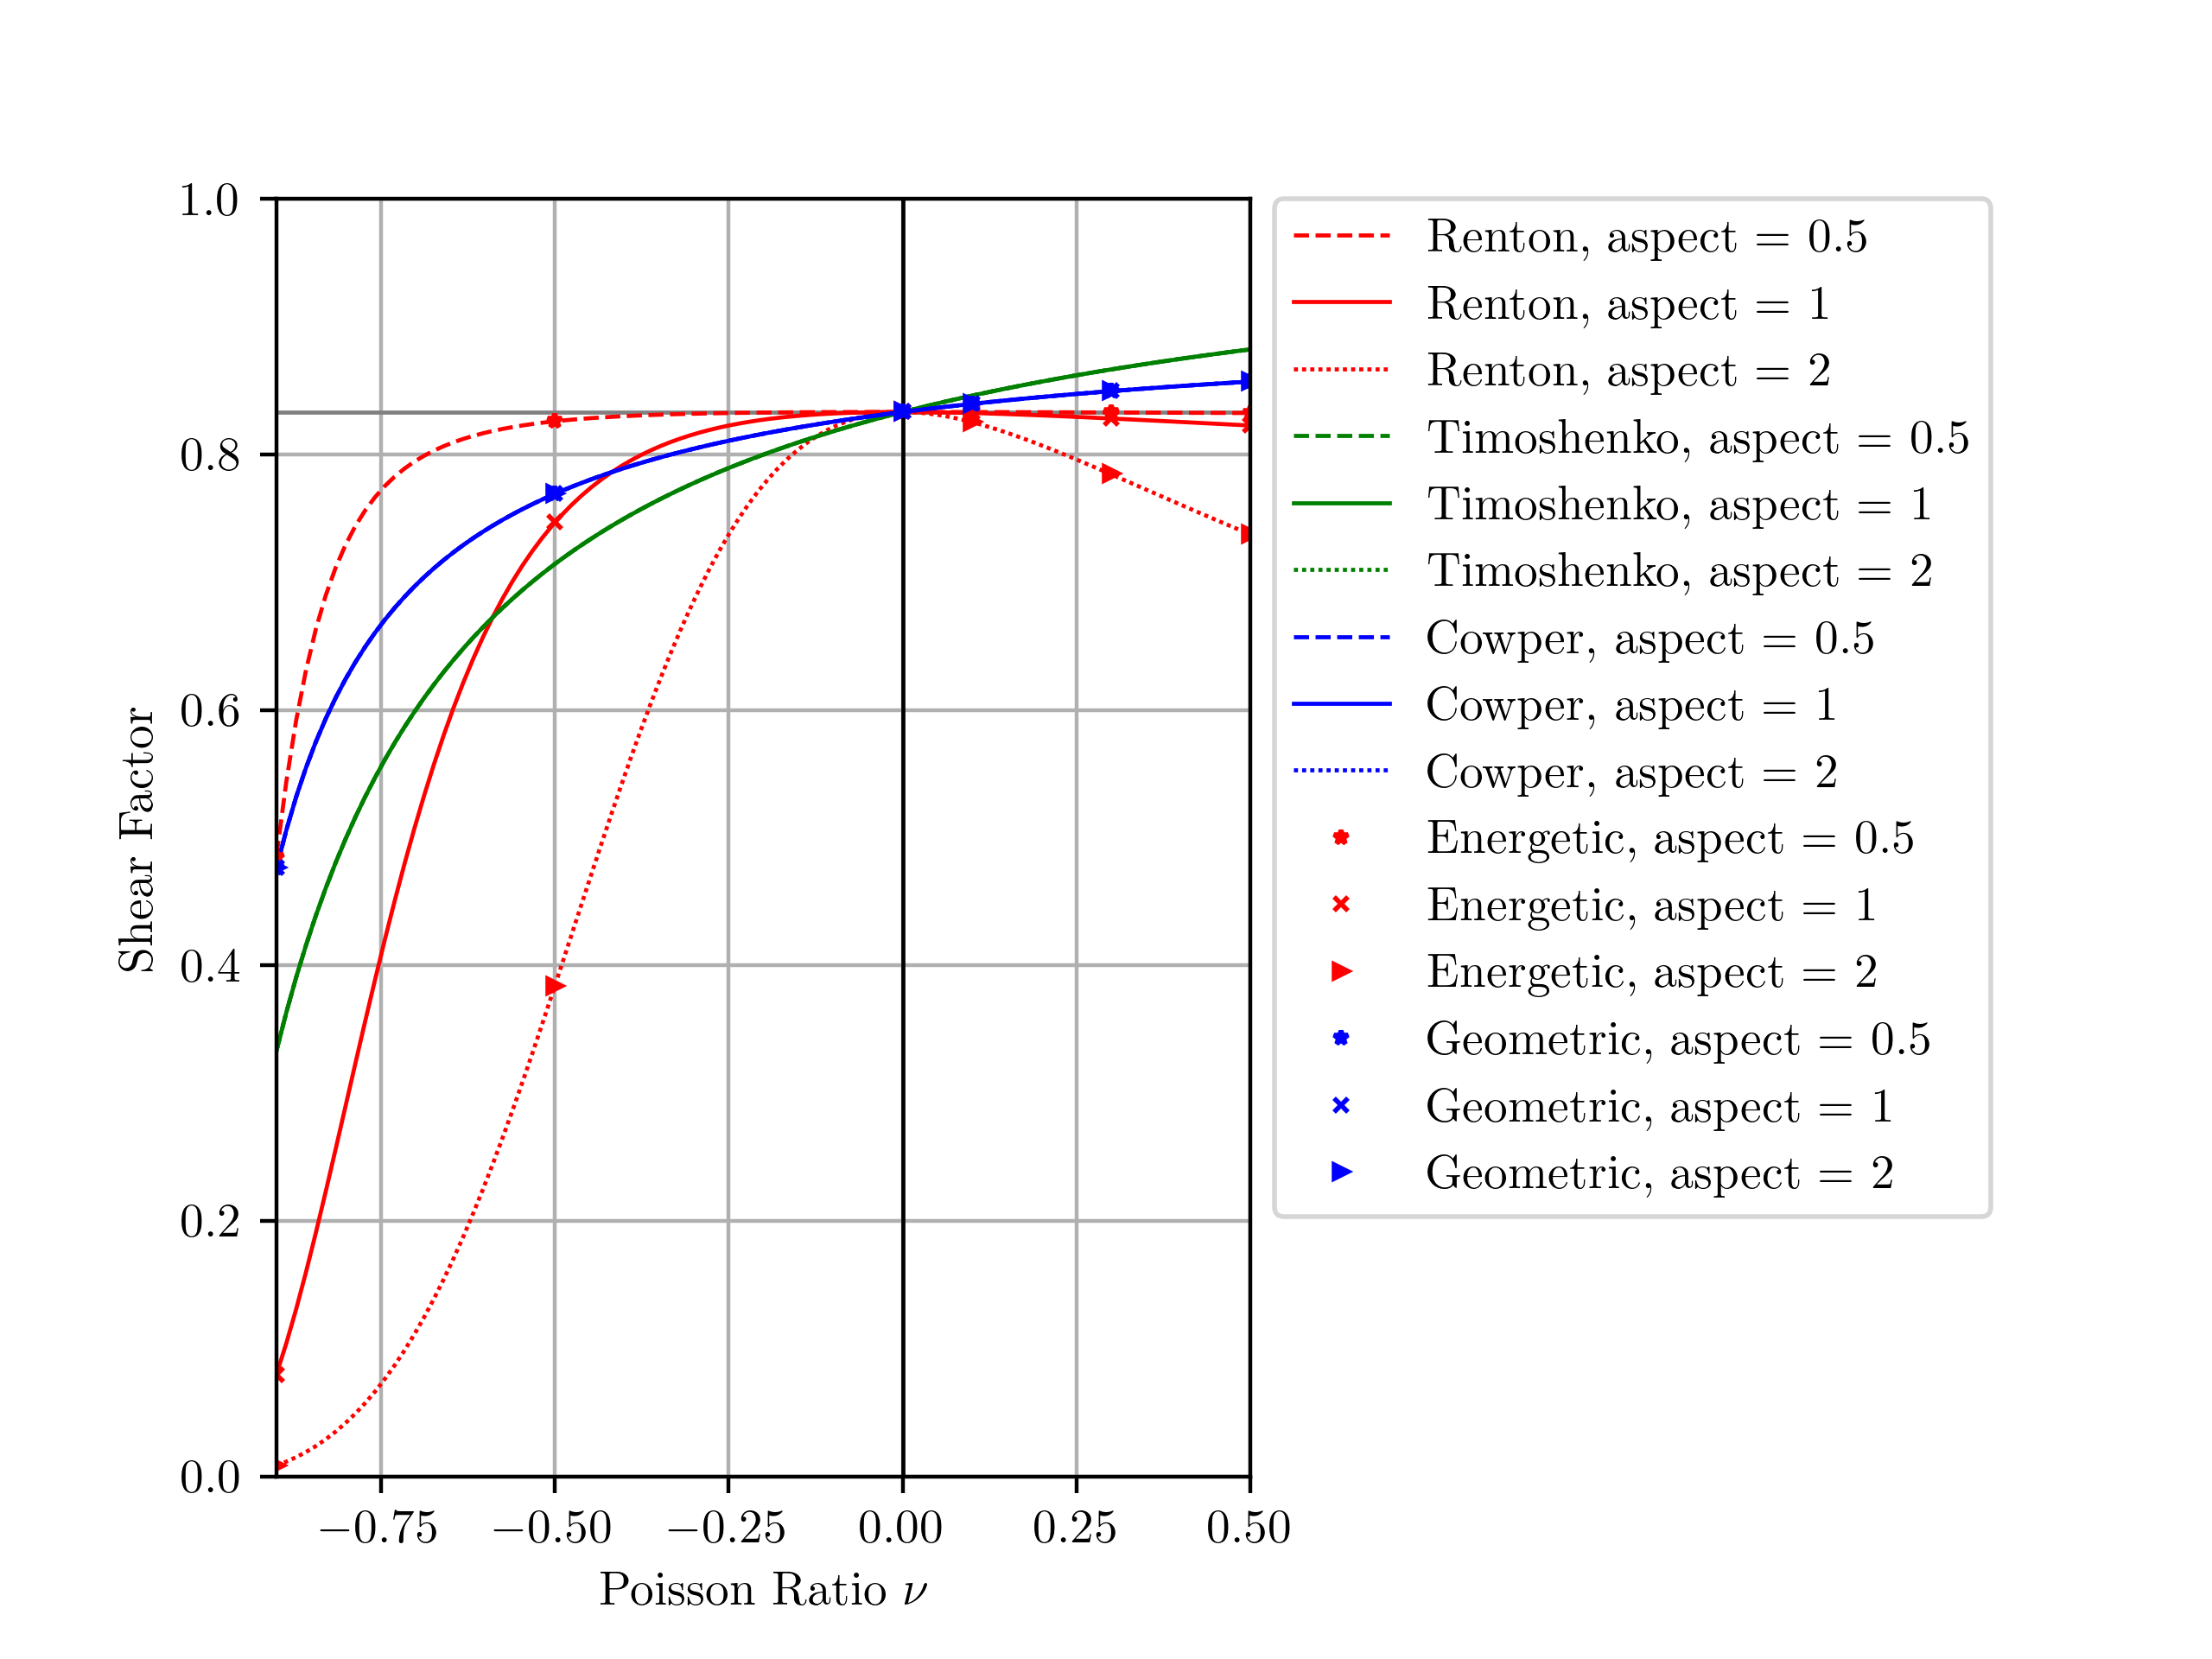
\includegraphics[width=0.8\linewidth]{Examples/frame-0012/img/shear_rectangle_poisson.png}
    \caption{Caption}
    \label{fig:0012-r}
\end{figure}


\subsubsection{Hollow Rectangle}\label{sec:frame-0012/H}

\begin{figure}[H]
  \centering 
  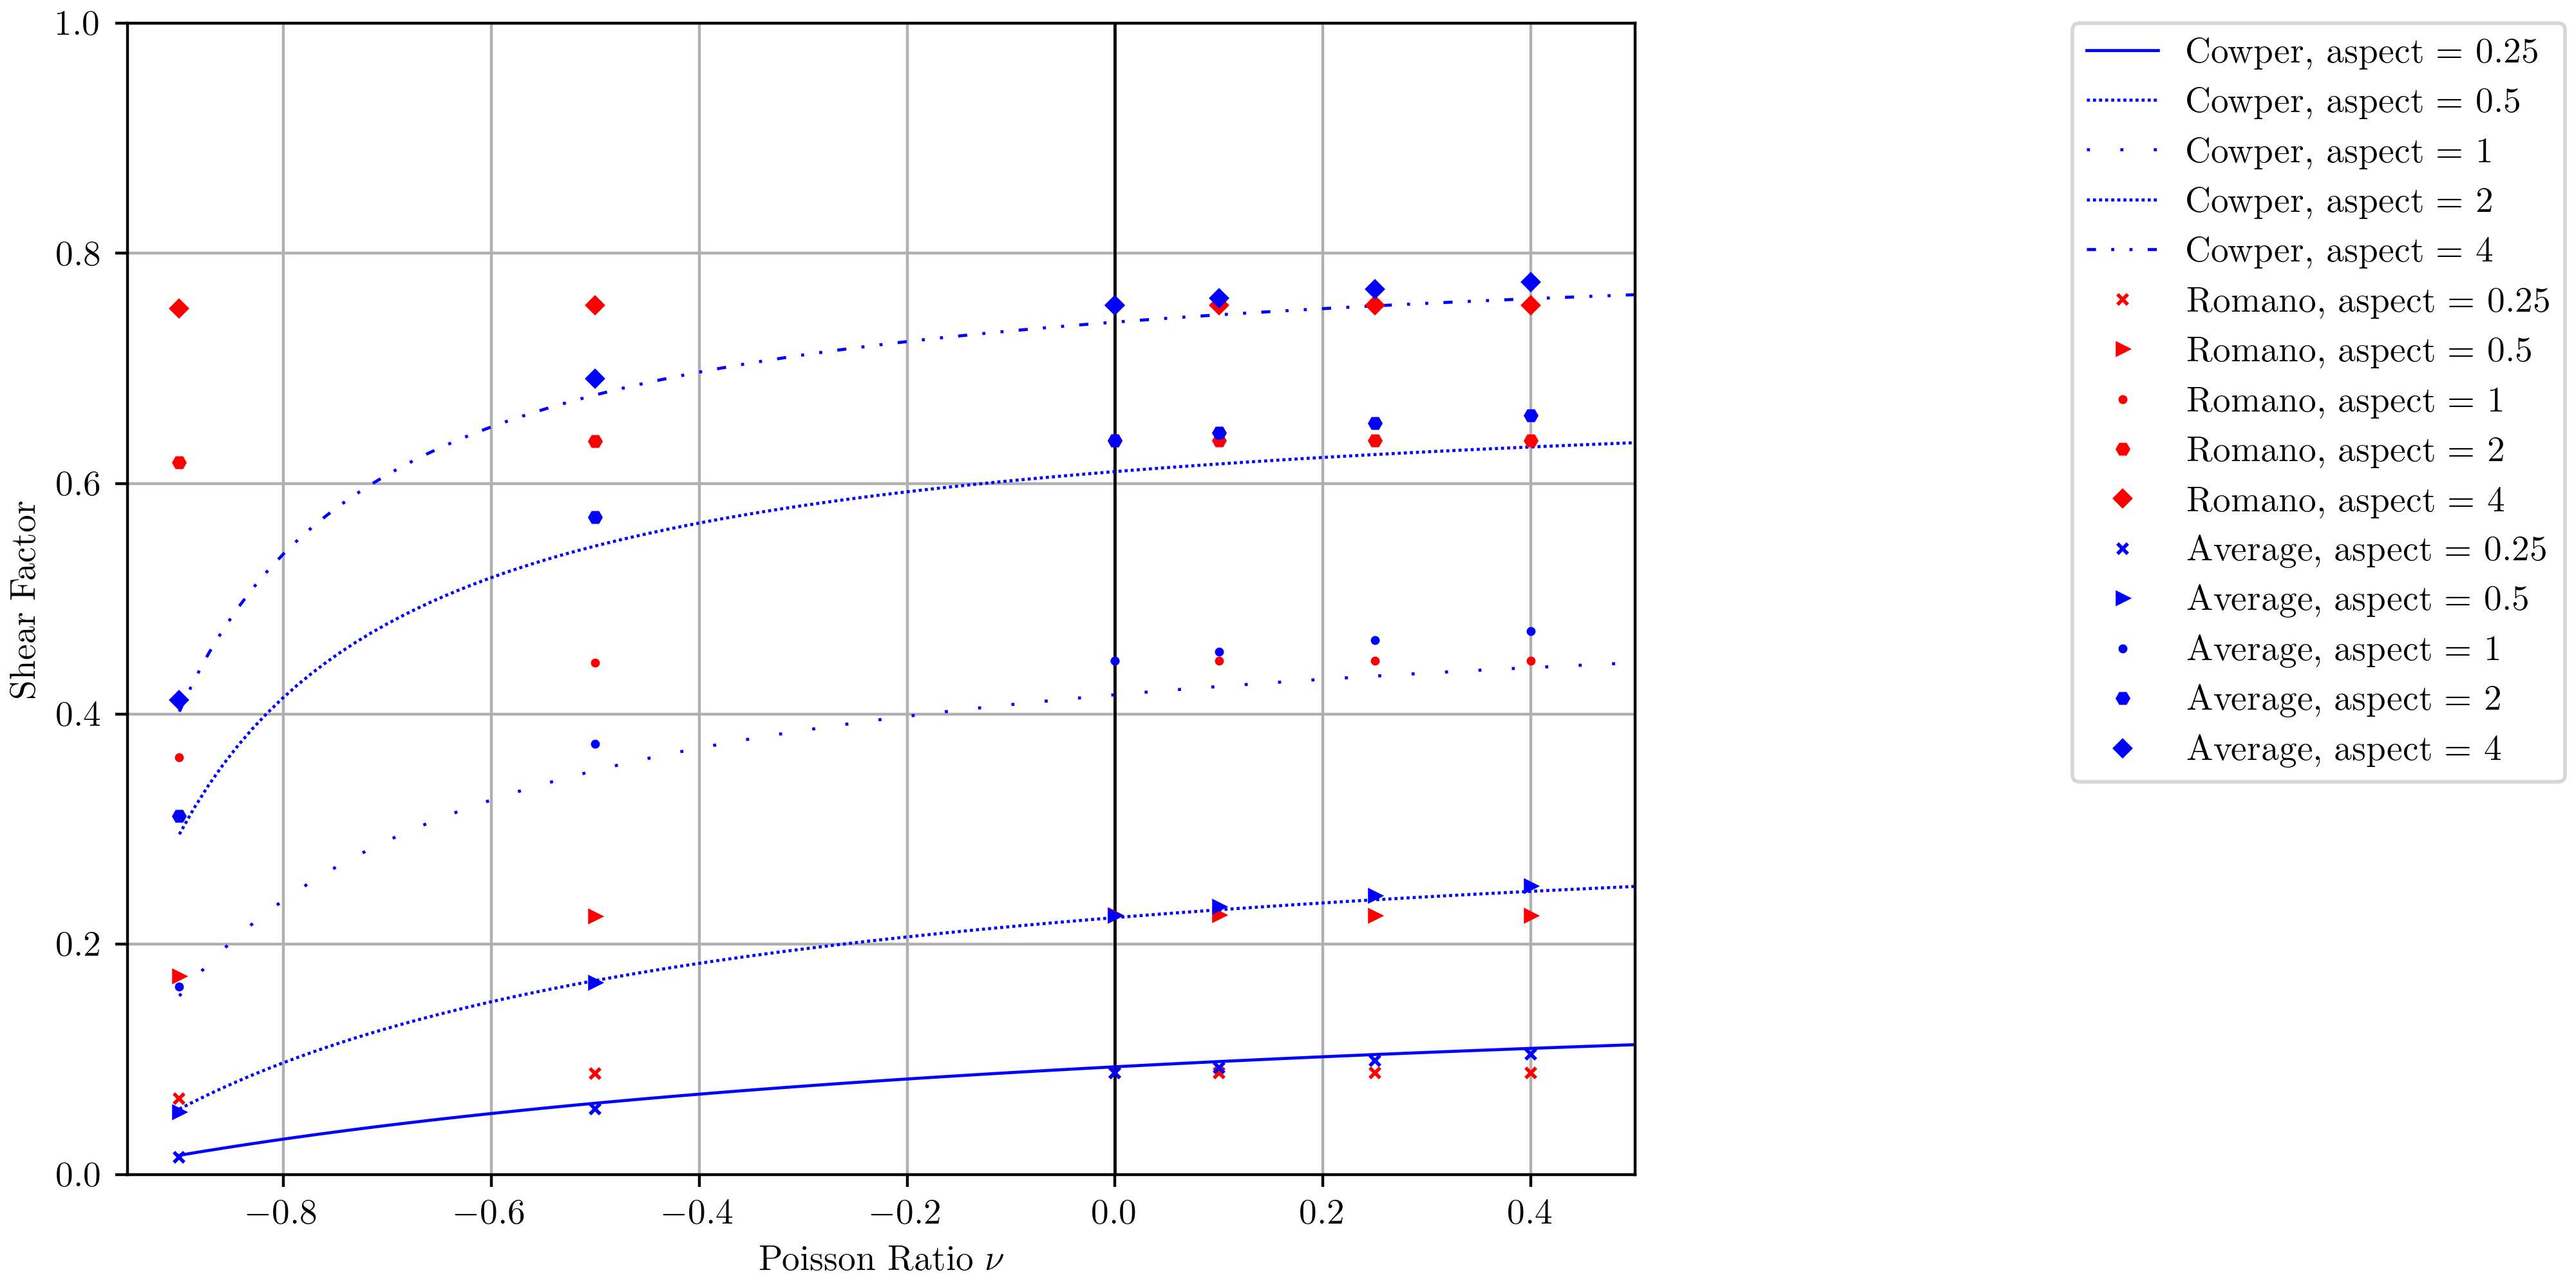
\includegraphics[width=0.8\linewidth]{Examples/frame-0012/img/shear_h_poisson.png}
\end{figure}



% \begin{figure}[H]
%     \centering
%     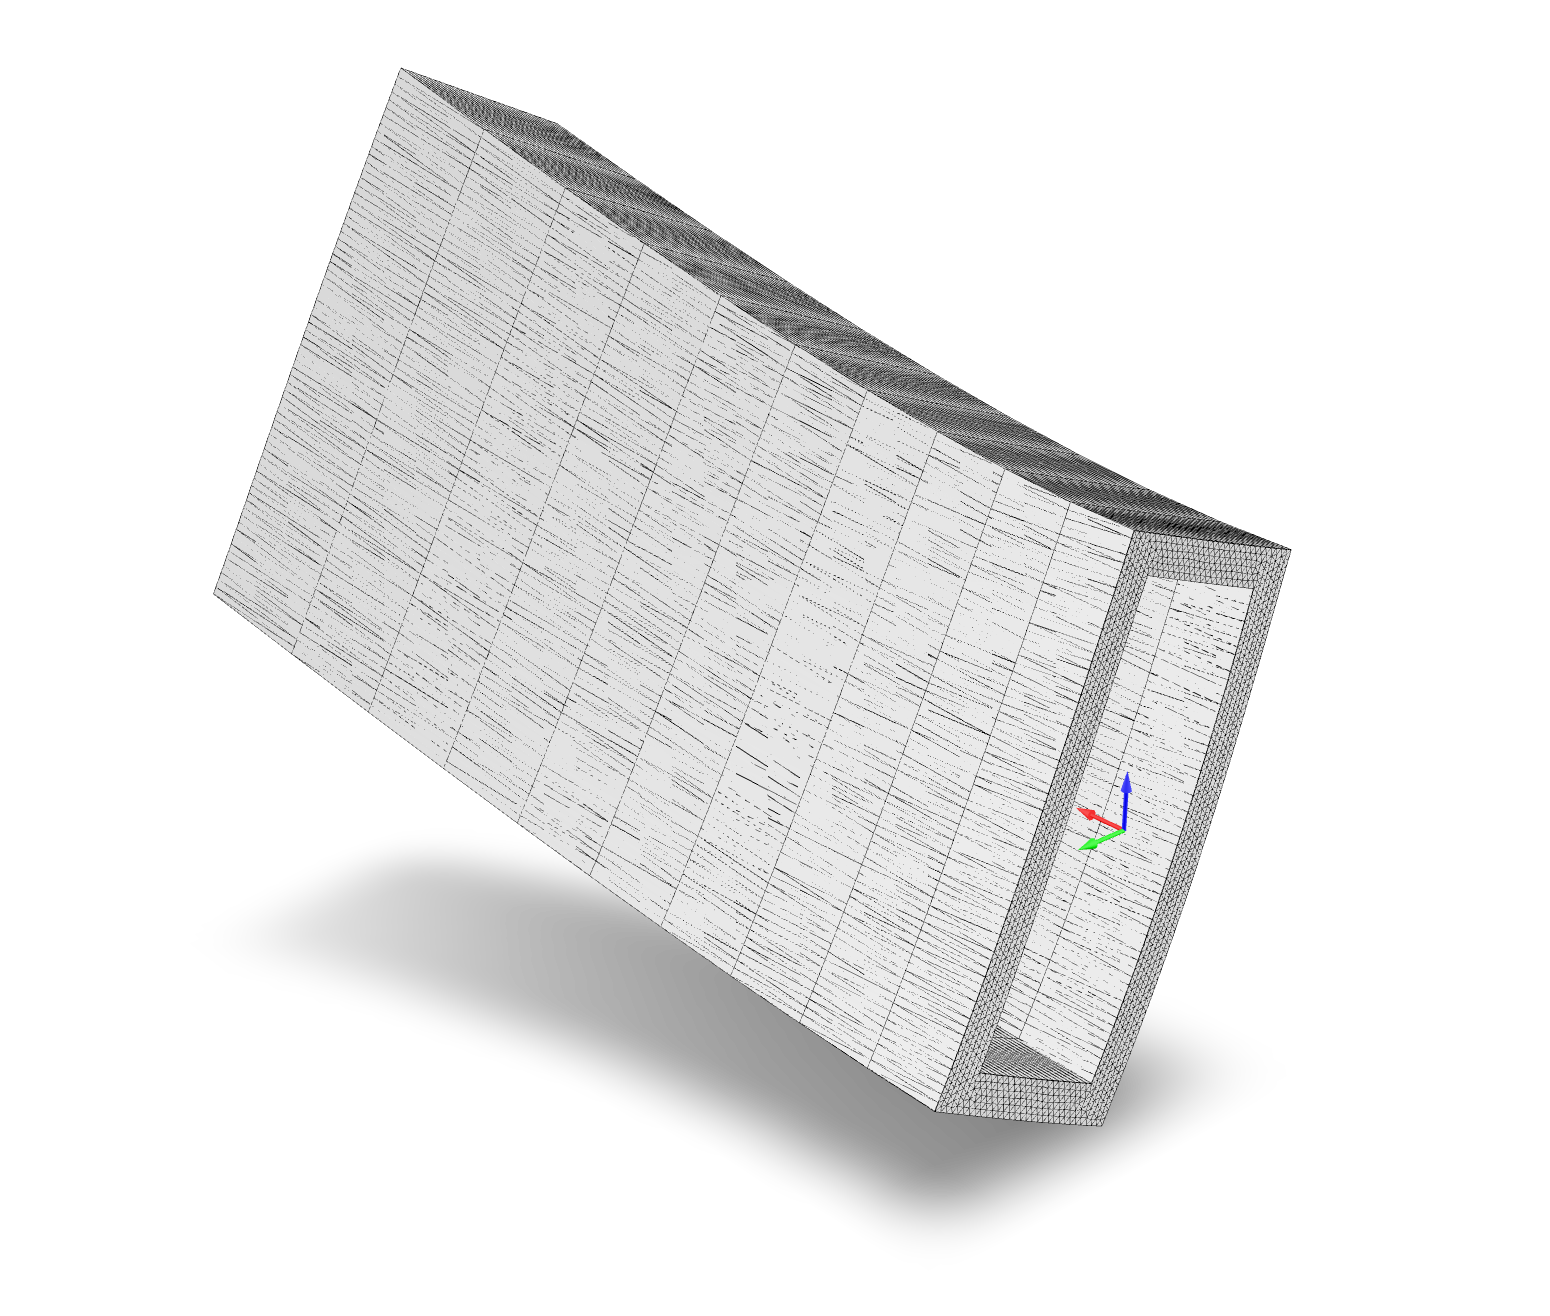
\includegraphics[width=0.5\linewidth]{Examples/frame-0012/img/0012-tube-soln.png}
%     \caption{Continuum solution from Example~\ref{sec:frame-0012/H}}
%     \label{fig:0012-tube}
% \end{figure}

